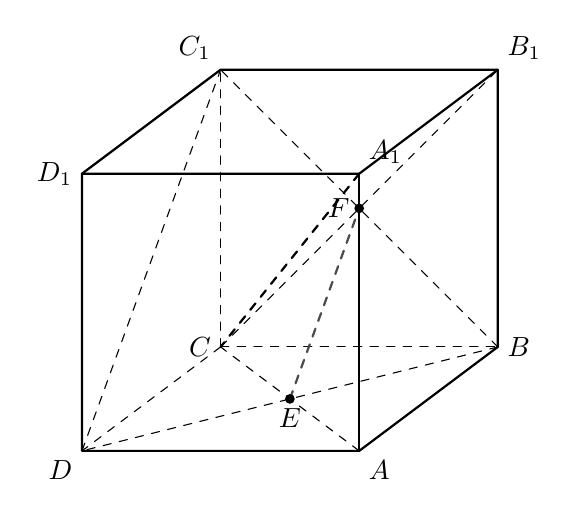
\begin{tikzpicture}[scale=2.2, line join=round, line cap=round, >=stealth]
  % 顶点坐标设定（斜二测投影）
  \coordinate (C) at (0, 0);
  \coordinate (D) at (-0.8, -0.6);
  \coordinate (A) at (0.8, -0.6);
  \coordinate (B) at (1.6, 0);

  \coordinate (C1) at (0, 1.6);
  \coordinate (D1) at (-0.8, 1.0);
  \coordinate (A1) at (0.8, 1.0);
  \coordinate (B1) at (1.6, 1.6);

  % 交点坐标
  \coordinate (E) at (0.4, -0.3); % AC 与 BD 交点
  \coordinate (F) at (0.8, 0.8);  % C1B 与 CB1 交点

  % 虚线部分（内部与后侧）
  \draw[dashed, thin] (C) -- (D);
  \draw[dashed, thin] (C) -- (B);
  \draw[dashed, thin] (C) -- (C1);
  \draw[dashed, thin] (A) -- (C);
  \draw[dashed, thin] (B) -- (D);
  \draw[dashed, thin] (C) -- (B1);
  \draw[dashed, thin] (B) -- (C1);
  \draw[dashed, thick] (A1) -- (C);
  \draw[dashed, thin] (D) -- (C1);
  \draw[dashed, thick, black!70] (E) -- (F);

  % 实线部分（外轮廓与前侧）
  \draw[thick] (D) -- (A) -- (B) -- (B1) -- (C1) -- (D1) -- cycle;
  \draw[thick] (A) -- (A1);
  \draw[thick] (D1) -- (A1) -- (B1);

  % 顶点标注
  \node[left] at (C) {$C$};
  \node[below left] at (D) {$D$};
  \node[below right] at (A) {$A$};
  \node[right] at (B) {$B$};
  \node[above left] at (C1) {$C_1$};
  \node[left] at (D1) {$D_1$};
  \node[above right] at (A1) {$A_1$};
  \node[above right] at (B1) {$B_1$};
  \node[below] at (E) {$E$};
  \node[left] at (F) {$F$};

  % 关键点标记
  \fill (E) circle (0.8pt);
  \fill (F) circle (0.8pt);
\end{tikzpicture}
